\documentclass[a4paper, 12pt]{book} % changed from scrbook
% not using \documentclass[a4paper, twoside=semi]{scrreprt} anymore

\usepackage{../Files/Style/InfoSec}

\definecolor{bg}{RGB}{20,20,20}
\definecolor{fg}{RGB}{220,220,220}
\definecolor{keyword}{RGB}{130,170,255}
\definecolor{comment}{RGB}{120,120,120}
\definecolor{string}{RGB}{255,200,120}

\lstdefinestyle{darkbash}{
    backgroundcolor=\color{bg},
    basicstyle=\scriptsize\ttfamily\color{fg},
    keywordstyle=\color{keyword},
    commentstyle=\color{comment},
    autogobble=true,
    stringstyle=\color{string},
    breaklines=true,
    showstringspaces=false,
    frame=single
}

% \usepackage{titlesec}
% \setkomafont{chapter}{\Huge\bfseries}
% \setkomafont{section}{\Large\bfseries}
% \setkomafont{subsection}{\large\bfseries}
\usepackage{fancyhdr, lastpage}
\usepackage{lstautogobble}
\usepackage{euscript}


\makeatletter
\providecommand{\subtitle}[1]{\gdef\@subtitle{#1}}
\providecommand{\@subtitle}{}
\makeatother


\usepackage{booktabs}
\usepackage{array}
\usepackage{multirow}




\usepackage{newfloat}
%\usepackage{tocloft}

% % Define new float environment
% \DeclareFloatingEnvironment[
%   fileext=lof,
%   listname={List of Flowcharts},
%   name=Flowchart,
% ]{flowchart}


\pagestyle{fancy}
%\fancyhf{}
\lhead{}
\chead{}
%\rhead{Introduction to the Theory of Computation}
\cfoot{\thepage\ of \pageref{LastPage}}
\rfoot{Version 8.3}




\RequirePackage{etex} 


%--- The documentation for the title can be found at: https://en.wikibooks.org/wiki/LaTeX/Title_Creation
\title{Information Security \\ Transport Layer Security}
\author{Ahmed U. Ashraf}
\date{\today }
% \subtitle{Version~\version}

\begin{document}

% \include{glossary}


\maketitle
%--- we would like to hyperlink each item in contensts page
% \let\hypercontentsline=\contentsline
% \renewcommand{\contentsline}[4]{\hypertarget{toc.#4}{}\hypercontentsline{#1}{#2}{#3}{#4}}
%--- We print ToC: Table of Contents

\DeclareFontShape{U}{stmry}{b}{n}{<-> ssub * stmry/m/n}{}

\tableofcontents\label{toc}
%--- We print the list of figures, this might go at the end.




% \listoffigures
% %--- We print the list of tables, this might also go at the end.
% \listoftables
% %--- This is to add list of symbols as glossary
% % \printunsrtglossary[type=symbols,style=long,title={List of Symbols}]


% % List of Algorithms (- taken the idea from Discrete Algorithmic Mathematics by Stephen B.Maurer and ANthony Ralston.pdf)

% \listofalgorithms
% \addcontentsline{toc}{chapter}{List of Algorithms}

% \listofflowcharts
% %\addcontentsline{toc}{chapter}{List of Flowcharts}


\newpage







\chapter{Introduction}




The \emph{Transport Layer Security} (TLS) is a widely used cryptographic protocol designed to provide secure communications over a computer network. Most commonly recognized as the technology behind HTTPS, TLS ensures 
\begin{enumerate}
    \item \emph{Data privacy} using symmetric encryption: RSA or DHE for passing keys.
    \item \emph{Authenticity} using RSA and PKI.
    \item \emph{Data Integrity}: In TLS 1.2 using MAC. In TLS 1.3 using Authenticated Encryption with Associated Data (AEAD) algorithms.
\end{enumerate}
between client and server. TLS protocol starts after TCP connection. 

\begin{longtable}{|c|c|c|}\hline 
    Name/Version & Year & Status \\ \hline
    SSL 1.0 & 1995 & flawed \\ \hline
    SSL 2.0 & 1995 & flawed \\ \hline 
    SSL 3.0 & 1996 & deprecated  (2015) \\ \hline 
    TLS 1.0 & 1999 & deprecated (2021) \\ \hline 
    TLS 1.1 & 2006 & deprecated (2021) \\ \hline 
    TLS 1.2 & 2008 & discouraged \\ \hline 
    TLS 1.3 & 2018 & current \\ \hline 
    \caption{History of TLS}
\end{longtable}

\section{TLS 1.2}
Here are the steps for handshake: 
\begin{enumerate}
    \item The client sends \verb|ClientHello|$= (\mathscr{S}, r_A, k_A)$, where $\mathscr{S}$ are supported cipher suites, $r_A$ is nonce, and $k_A = g^a$ is a client DH key.
    \item The server sends \verb|ServerHello|$= (\mathrm{S}, r_B, k_B)$, where $\mathrm{S}$ is a chosed cipher suite, $r_B$ is a nonce, and $k_B = g^b$ is a server DH key.
\end{enumerate}
At the end of this both has a shared secret $s = g^{ab}$. From this point onwards, the messages are encrypted.
\begin{enumerate}
    \item Server sends certificate (that also contains public parameters for authentication).
    \item 
\end{enumerate}


\chapter{TLS 1.3}

\begin{enumerate}
    \item The \verb|ClientHello| consists of:
    \begin{enumerate}
        \item Protocol version.
        \item Pre-computed public key material.
        \item Signatures.
    \end{enumerate}
    \item The \verb|ServerHello| consists of:
    \begin{enumerate}
        \item The accepted cipher suite.
        \item The accepted key exchange.
    \end{enumerate}
\end{enumerate}

Note that TLS  1.3 have only 5 recommended suites
\begin{enumerate}
    \item \verb|TLS_AES_256_GCM_SHA384|: Uses 256-bit AES for bulk encryption in GCM and SHA-384 for message integrity.
    \item \verb|TLS_CHACHA20_POLY1305_SHA256|: Uses ChaCha20 encryption algorithm and Poly1305 for authentication.
    \item \verb|TLS_AES_128_GCM_SHA256|: Uses 128-biit AES for encryption and SHA-256 for message integrity.
    \item \verb|TLS_AES_128_CCM_SHA256|: utilises CCM.
    \item \verb|TLS_AES_128_CCM_8_SHA256|: CCM mode that truncates the authentication to 8 bytes.
\end{enumerate}



% \begin{figure}[H]
%     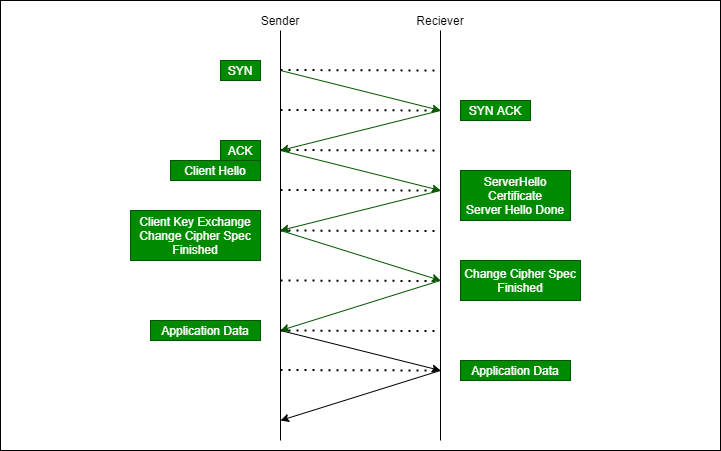
\includegraphics[scale=0.7]{tlsdiagram.png}
% \end{figure}




\section{Cipher Suites}

A cipher suite (for TLS1.2) looks like
\begin{center}
        \verb|TLS_ECDHE_ECDSA_WITH_AES_128_GCM_SHA256|    
\end{center}
It contains:
\begin{enumerate}
    \item Protocol: Transport Layer Security (TLS).
    \item Secret Key Exchange: Elliptic Curve Diffie Hellman Ephemeral (ECDHE).
    \item Public Key Authentication Method: Elliptic Curve Digital Signature Algorithm (ECDSA).
    \item AEAD Cipher: Advanced Encyrption Standard (AES) with key size 128bits with operations of GCM.
    \item PRF Hash algorithm: SHA256.
\end{enumerate}
So we can read it as 
\begin{center}
    Use Ephemeral Elliptic-Curve Diffie-Hellman (ECDHE) to establish a shared secret, authenticate the server using ECDSA signatures, encrypt all traffic using AES-128 in GCM mode, and use SHA-256 during the TLS 1.2 key-derivation and handshake process.
\end{center}

A cipher suite (for TLS1.3) looks like
\begin{center}
    \verb|TLS_AES_256_GCM_SHA384|
\end{center}
It contains:
\begin{enumerate}
    \item Protocol: Transport Layer Security (TLS).
    \item Secret Key Exchange: Elliptic Curve Diffie Hellman Ephemeral (ECDHE).
    \item Public Key Authentication Method: Elliptic Curve Digital Signature Algorithm (ECDSA).
    \item AEAD Cipher: Advanced Encyrption Standard (AES) with key size 128bits with operations of GCM.
    \item PRF Hash algorithm: SHA256.
\end{enumerate}










% \chapter{References}

%-- Computation Engineering by Ganesh Gopalakrishnan

\cite{adamson2012set}

% \nocite{*}    



\bibliography{../Bibliography/references}
\bibliographystyle{amsalpha}

\printindex




\end{document}